% Chapter 1

\chapter{Results and Conclusions} % Main chapter title

\label{Chapter3} % For referencing the chapter elsewhere, use \ref{Chapter1} 

\lhead{Chapter 3. \emph{Results and Conclusions}} % This is for the header on each page - perhaps a shortened title

%----------------------------------------------------------------------------------------

The results were obtained using Floquet Analysis for a system with $j=10, p1=p2=\frac{1}{j}, K1=K1=1$ and are plotted against that obtained using Dalibard's Analysis. The plots are shown on the following two pages.

We can see from the plots that $S_v$ both the Dalibard and Floquet results match at low $\epsilon$ values and both these values tend to zero, as is expected for this $\epsilon$ range. The results also match for $\epsilon = 1$, which itself is a pretty high value of coupling. As we increase our $\epsilon$ value above 1, we can see that the Dalibard method breaks down. This is majorly because our method is an approximation, and the terms in the $H_{eff}$ of our system break down at higher values of $\epsilon$.

\begin{figure}[p]
\centering
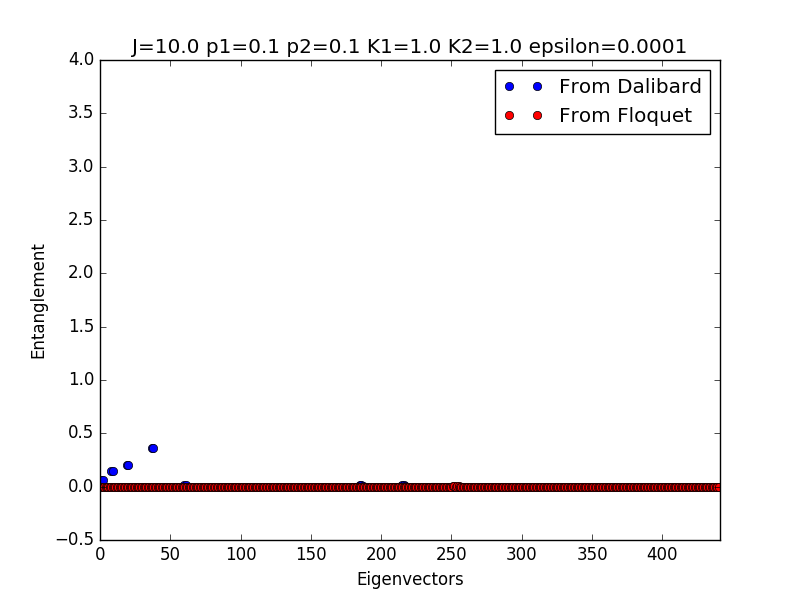
\includegraphics[width=0.5\textwidth]{Figures/epsilon_0_0001.png}
\end{figure}

\begin{figure}[p]
\centering
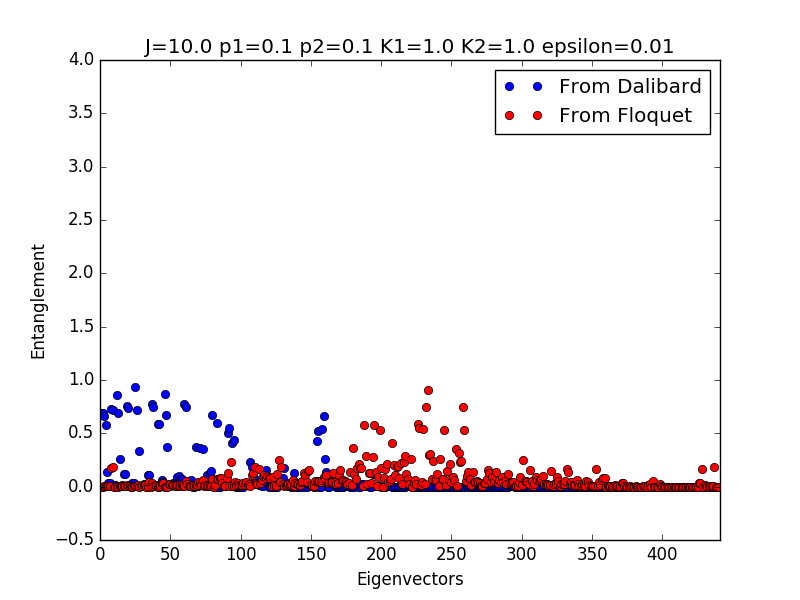
\includegraphics[width=0.5\textwidth]{Figures/epsilon_0_01.png}
\end{figure}

\begin{figure}[p]
\centering
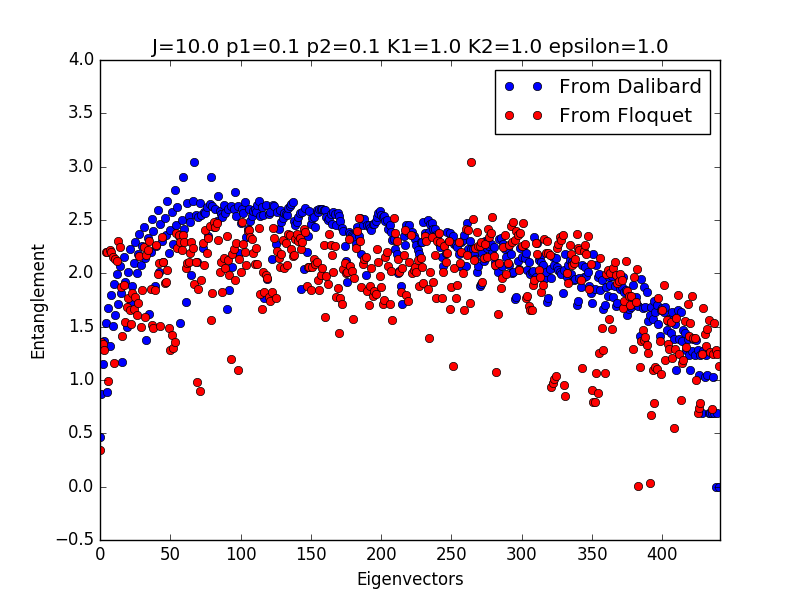
\includegraphics[width=0.5\textwidth]{Figures/epsilon_1.png}
\end{figure}

\begin{figure}[p]
\centering
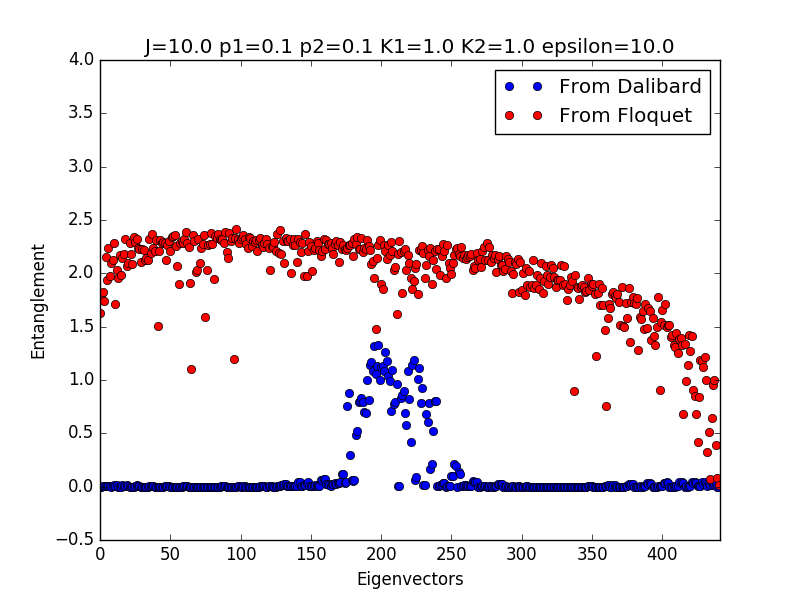
\includegraphics[width=0.5\textwidth]{Figures/epsilon_10.png}
\end{figure}

\begin{figure}[p]
\centering
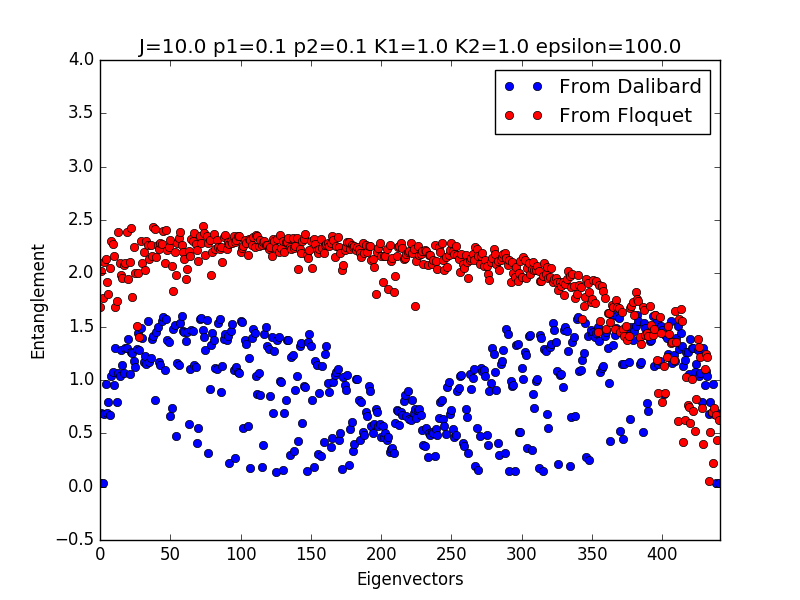
\includegraphics[width=0.5\textwidth]{Figures/epsilon_100.png}
\end{figure}

\begin{figure}[p]
\centering
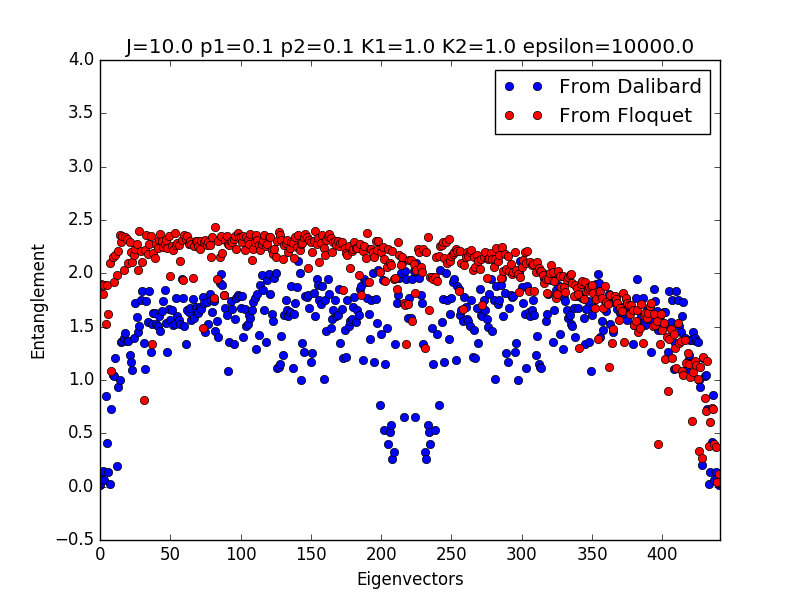
\includegraphics[width=0.5\textwidth]{Figures/epsilon_10000.png}
\end{figure}

